
\begin{figure}[t]
\centering

\begin{subfigure}[b]{0.31\textwidth}
  \centering    
  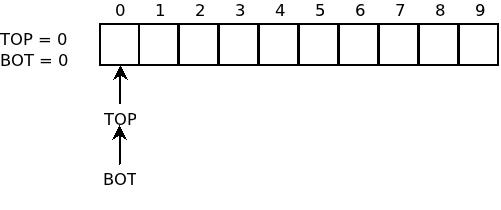
\includegraphics[width=\textwidth]{circ-init}
  \caption{
     \tiny The initial state of the circular array.
  }
  \label{fig:circ-1}
\end{subfigure}
~ %spacer
\begin{subfigure}[b]{0.31\textwidth}
  \centering
  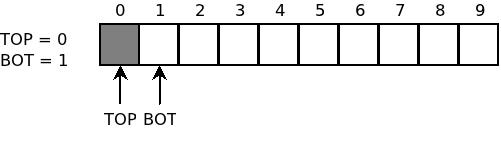
\includegraphics[width=\textwidth]{circ-push1}
  \vspace{1pt}
  \caption{
     \tiny The state after one de\_push\_bottom operation.
  }
  \label{fig:circ-2}
\end{subfigure}
~ %spacer
\begin{subfigure}[b]{0.31\textwidth}
  \centering
  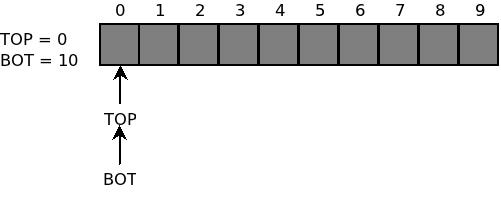
\includegraphics[width=\textwidth]{circ-push2}
  \caption{
    \tiny After a further nine de\_push\_bottom operations. 
  }
  \label{fig:circ-3}
\end{subfigure}

\vspace{10pt}

\begin{subfigure}[b]{0.31\textwidth}
  \centering
  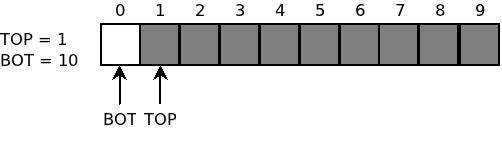
\includegraphics[width=\textwidth]{circ-steal1}
  \caption{
    \tiny After one de\_steal operation.
  }
  \label{fig:circ-4}
\end{subfigure}
~ %spacer
\begin{subfigure}[b]{0.31\textwidth}
  \centering
  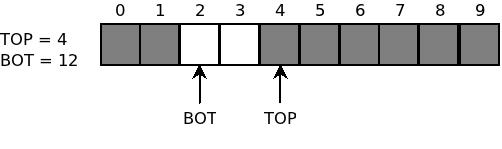
\includegraphics[width=\textwidth]{circ-stealpush1}
  \caption{
    \tiny After three more de\_steal operations followed by two de\_push\_bottom
          operations.
  }
  \label{fig:circ-5}
\end{subfigure}
~ %spacer
\begin{subfigure}[b]{0.31\textwidth}
  \centering
  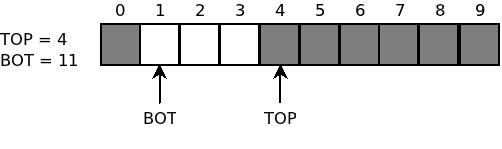
\includegraphics[width=\textwidth]{circ-pop1}
  \caption{
    \tiny After one de\_pop\_bottom operation.
  }
  \label{fig:circ-6}
\end{subfigure}

% full caption
\caption{
    A demonstration of the a sequence of operations applied to the circular array
    data-structure.
    The `TOP' field refers to the index of the top element of the deque and
    the `BOT' field refers to the index of the bottom element plus one.
    White squares indicate an un-used element, shaded squares indicate
    elements which are in use.
}
\label{fig:circ-demo}
\end{figure}

